\documentclass[12pt]{article}

% ---------- Paquetes ----------
\usepackage[utf8]{inputenc}
\usepackage[T1]{fontenc}
\usepackage[provide=*,spanish]{babel}
\usepackage{helvet}          % Fuente tipo Arial
\renewcommand{\familydefault}{\sfdefault}
\usepackage[margin=2.5cm]{geometry}
\usepackage{graphicx}
\usepackage{amsmath}
\usepackage{amssymb}
\usepackage{booktabs}
\usepackage{array}
\usepackage[table]{xcolor}   % se usa solo para blanco/negro, sin colores extra
\usepackage{titlesec}
\usepackage{enumitem}
\usepackage{hyperref}

% Todo en color negro, sin colores adicionales
\hypersetup{
    colorlinks=false,
    pdfborder={0 0 0}
}
\color{black}

% Formato de secciones: negro, sin color extra
\titleformat{\section}
  {\normalfont\fontsize{14}{16}\bfseries\color{black}}
  {\thesection}{1em}{}

\setlength{\parindent}{0pt}
\setlength{\parskip}{6pt}

\begin{document}

% ================= PORTADA =================
\begin{titlepage}
\centering
\vspace*{0.5cm}


\includegraphics[width=0.95\textwidth]{images/logos/utvam_logo.png}

\vspace{0.4cm}

\begin{minipage}{0.45\textwidth}
\centering

\includegraphics[height=1.4cm]{images/logos/sep_logo.png}
\end{minipage}
\hfill
\begin{minipage}{0.45\textwidth}
\centering

\includegraphics[height=1.4cm]{images/logos/utp_logo.png}
\end{minipage}

\vspace{2cm}

{\Huge \textbf{CÁLCULO DE VARIAS VARIABLES}}

\vspace{1.5cm}

{\Large \textbf{E.D. 1.1. Funciones Escalares de Varias Variables}}

\vspace{2.5cm}

{\large
Radamontes Peniche Joseph Ivan\\
Martinez Pioquinto Siedfried Miguel\\
Jiménez Lopez Pablo Jesús\\
TID 401
}

\vspace{2cm}

{\large \textbf{Docente: Rubén Ramírez Gómez}}

\vfill

{\large \textbf{Septiembre, 2026}}

\end{titlepage}

% ================= CONTENIDO =================

% ---------------- Ejercicio 1 ----------------
\section*{Ejercicio 1: El ``Círculo de Cobertura'' (Raíz Cuadrada)}
\[ f(x,y) = \sqrt{16 - x^2 - y^2} \]

\textbf{Representación Verbal:} La intensidad de señal Wi-Fi alcanza su valor máximo de 4 unidades en el origen $(0,0)$ y disminuye simétricamente hasta hacerse 0 a una distancia de 4 unidades del centro.

\textbf{Variables:}
\begin{itemize}[nosep]
    \item Independientes: $x$ (GPS X), $y$ (GPS Y)
    \item Dependiente: $f(x,y)$ o $z$ (Intensidad Wi-Fi)
\end{itemize}

\textbf{Dominio y Rango:}
\begin{itemize}[nosep]
    \item Dominio: $D = \{(x,y) \in \mathbb{R}^2 \mid x^2 + y^2 \leq 16\}$
    \item Rango: $R = [0,4]$
\end{itemize}

\textbf{Representación Algorítmica (Tabular):} \quad $z = \sqrt{16-x^2-y^2}$

\begin{center}
\begin{tabular}{ccc}
\toprule
$x$ & $y$ & $f(x,y)$ \\
\midrule
0 & 0 & 4 \\
0 & 4 & 0 \\
2 & 2 & $\sqrt{8} \approx 2.83$ \\
\bottomrule
\end{tabular}
\end{center}

\begin{center}
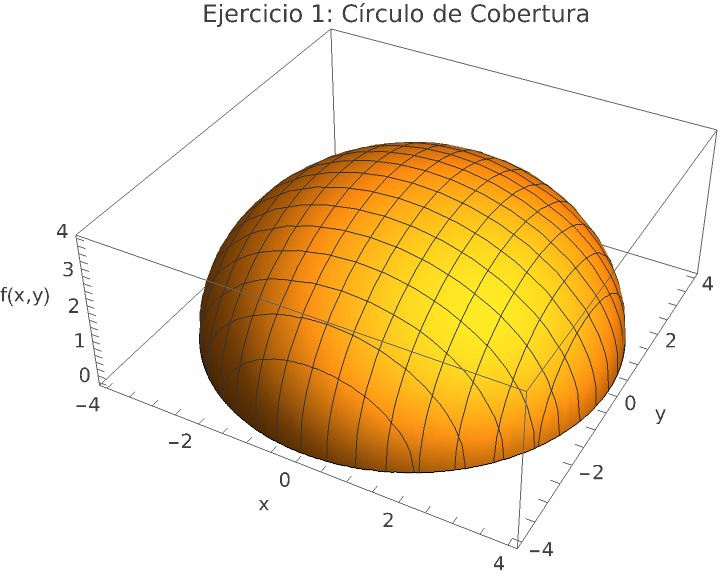
\includegraphics[width=0.75\textwidth]{images/Ejercicio1.png}
\end{center}

\newpage

% ---------------- Ejercicio 2 ----------------
\section*{Ejercicio 2: Latencia en Servidor de Metaverso (Racional)}
\[ L(d,c) = \dfrac{d}{100-c} \]

\textbf{Representación Verbal:} La latencia del servidor varía directamente proporcional a la distancia física $d$ e inversamente con respecto a la capacidad disponible $(100-c)$.

\textbf{Variables:}
\begin{itemize}[nosep]
    \item Independientes: $d$ (Distancia km), $c$ (Carga \%)
    \item Dependiente: $L$ (Latencia ms)
\end{itemize}

\textbf{Dominio y Rango:}
\begin{itemize}[nosep]
    \item Dominio: $D = \{(d,c) \in \mathbb{R}^2 \mid d \geq 0,\ 0 \leq c < 100\}$
    \item Rango: $R = [0, \infty)$
\end{itemize}

\textbf{Representación Algorítmica (Tabular):} \quad $L = \dfrac{d}{100-c}$

\begin{center}
\begin{tabular}{ccc}
\toprule
$d$ (km) & $c$ (\%) & $L(d,c)$ (ms) \\
\midrule
10 & 0 & 0.10 \\
50 & 50 & 1.00 \\
100 & 90 & 10.00 \\
\bottomrule
\end{tabular}
\end{center}

\begin{center}
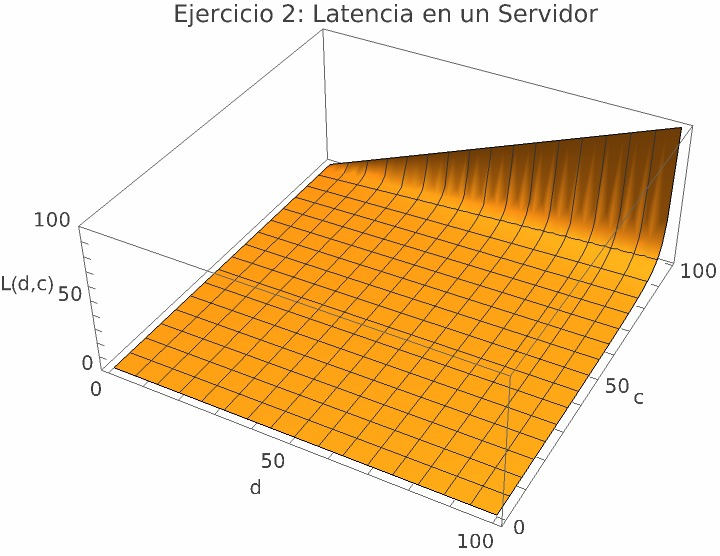
\includegraphics[width=0.75\textwidth]{images/Ejercicio2.png}
\end{center}

\newpage

% ---------------- Ejercicio 3 ----------------
\section*{Ejercicio 3: El ``Balanceador de Carga'' (Racional)}
\[ f(x,y) = \dfrac{100}{x+y} \]

\textbf{Representación Verbal:} El porcentaje de carga de trabajo disminuye a medida que aumenta la suma combinada de las capacidades operativas de ambos servidores.

\textbf{Variables:}
\begin{itemize}[nosep]
    \item Independientes: $x$ (Cap. Servidor 1), $y$ (Cap. Servidor 2)
    \item Dependiente: $f(x,y)$ (\% Carga de trabajo)
\end{itemize}

\textbf{Dominio y Rango:}
\begin{itemize}[nosep]
    \item Dominio: $D = \{(x,y) \in \mathbb{R}^2 \mid x+y \neq 0\}$, con $(x,y > 0)$
    \item Rango: $R = (0, \infty)$
\end{itemize}

\textbf{Representación Algorítmica (Tabular):} \quad $z = \dfrac{100}{x+y}$

\begin{center}
\begin{tabular}{ccc}
\toprule
$x$ & $y$ & $f(x,y)$ (\%) \\
\midrule
10 & 10 & 5 \\
25 & 25 & 2 \\
50 & 50 & 1 \\
\bottomrule
\end{tabular}
\end{center}

\begin{center}
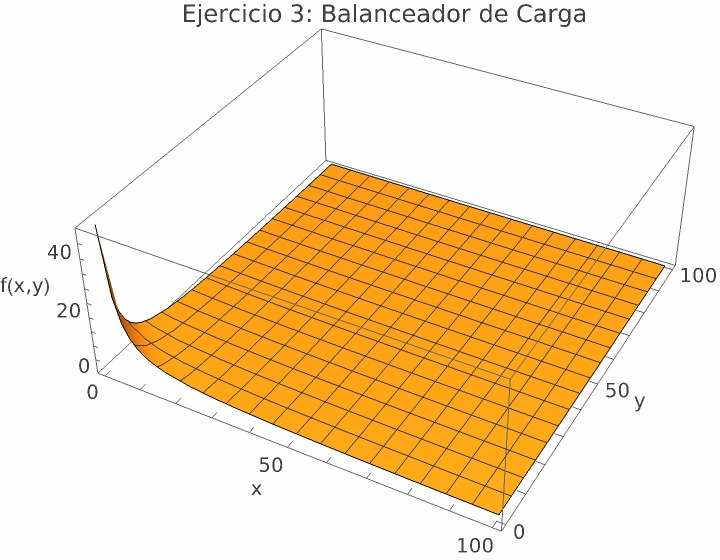
\includegraphics[width=0.75\textwidth]{images/Ejercicio3.png}
\end{center}

\newpage

% ---------------- Ejercicio 4 ----------------
\section*{Ejercicio 4: Calidad de Experiencia (QoE) en VR (Raíz)}
\[ Q(r,p) = \sqrt{r \cdot p} \]

\textbf{Representación Verbal:} El índice global de calidad se calcula como la media geométrica entre la tasa de refresco $r$ y la densidad de píxeles $p$ del visor VR.

\textbf{Variables:}
\begin{itemize}[nosep]
    \item Independientes: $r$ (Tasa refresco Hz), $p$ (Densidad píxeles)
    \item Dependiente: $Q$ (Índice Calidad QoE)
\end{itemize}

\textbf{Dominio y Rango:}
\begin{itemize}[nosep]
    \item Dominio: $D = \{(r,p) \in \mathbb{R}^2 \mid r\cdot p \geq 0\}$, con $(r,p \geq 0)$
    \item Rango: $R = [0, \infty)$
\end{itemize}

\textbf{Representación Algorítmica (Tabular):} \quad $Q = \sqrt{r \cdot p}$

\begin{center}
\begin{tabular}{ccc}
\toprule
$r$ (Hz) & $p$ (ppi) & $Q(r,p)$ \\
\midrule
60 & 60 & 60.00 \\
90 & 100 & $\sqrt{9000} \approx 94.87$ \\
120 & 120 & 120.00 \\
\bottomrule
\end{tabular}
\end{center}

\begin{center}
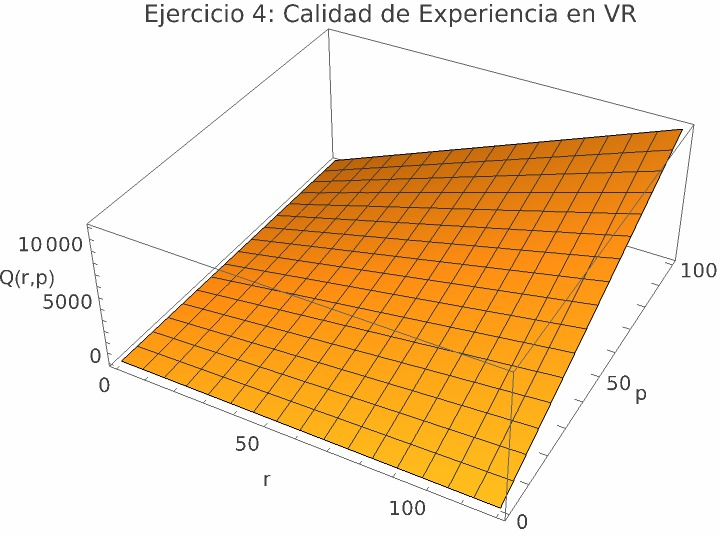
\includegraphics[width=0.75\textwidth]{images/Ejercicio4.png}
\end{center}

\newpage

% ---------------- Ejercicio 5 ----------------
\section*{Ejercicio 5: El ``Algoritmo Logarítmico'' (Logaritmo)}
\[ f(x,y) = \ln(y - x^2) \]

\textbf{Representación Verbal:} El tiempo de ejecución del algoritmo es proporcional al logaritmo natural del exceso de memoria respecto al cuadrado de la complejidad.

\textbf{Variables:}
\begin{itemize}[nosep]
    \item Independientes: $x$ (Complejidad), $y$ (Memoria)
    \item Dependiente: $f(x,y)$ (Tiempo de ejecución)
\end{itemize}

\textbf{Dominio y Rango:}
\begin{itemize}[nosep]
    \item Dominio: $D = \{(x,y) \in \mathbb{R}^2 \mid y > x^2\}$
    \item Rango: $R = (-\infty, \infty)$
\end{itemize}

\textbf{Representación Algorítmica (Tabular):} \quad $z = \ln(y - x^2)$

\begin{center}
\begin{tabular}{ccc}
\toprule
$x$ & $y$ & $f(x,y)$ \\
\midrule
0 & $e \approx 2.718$ & 1.00 \\
1 & 2 & $\ln(1) = 0.00$ \\
2 & 5 & $\ln(1) = 0.00$ \\
\bottomrule
\end{tabular}
\end{center}

\begin{center}
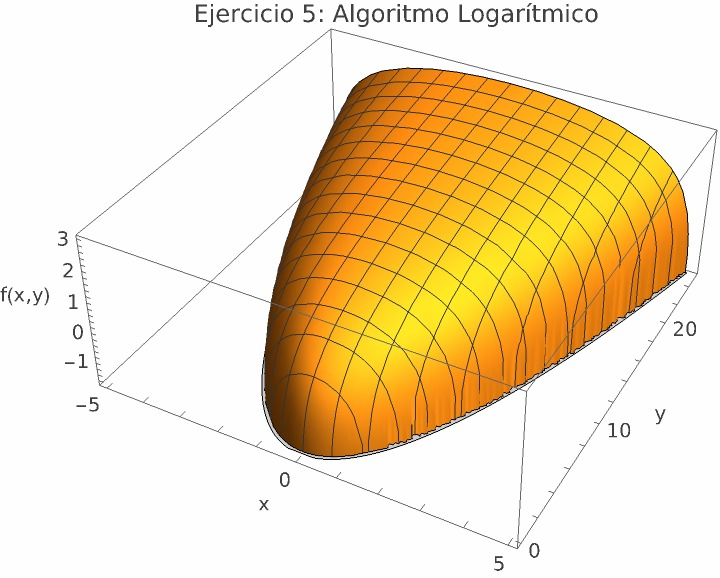
\includegraphics[width=0.75\textwidth]{images/Ejercicio5.png}
\end{center}

\newpage

% ---------------- Ejercicio 6 ----------------
\section*{Ejercicio 6: Utilidad Neta de Producto Digital (Logarítmica)}
\[ u(v,g) = \ln(v - g) \]

\textbf{Representación Verbal:} La utilidad percibida responde de forma logarítmica al beneficio neto generado (ventas totales menos costos de adquisición CAC).

\textbf{Variables:}
\begin{itemize}[nosep]
    \item Independientes: $v$ (Ventas totales \$), $g$ (Gastos CAC \$)
    \item Dependiente: $u$ (Utilidad percibida)
\end{itemize}

\textbf{Dominio y Rango:}
\begin{itemize}[nosep]
    \item Dominio: $D = \{(v,g) \in \mathbb{R}^2 \mid v > g\}$
    \item Rango: $R = (-\infty, \infty)$
\end{itemize}

\textbf{Representación Algorítmica (Tabular):} \quad $u = \ln(v-g)$

\begin{center}
\begin{tabular}{ccc}
\toprule
$v$ (\$) & $g$ (\$) & $u(v,g)$ \\
\midrule
100 & 99 & $\ln(1) = 0.00$ \\
1{,}000 & 900 & $\ln(100) \approx 4.61$ \\
5{,}000 & 1{,}000 & $\ln(4000) \approx 8.29$ \\
\bottomrule
\end{tabular}
\end{center}

\begin{center}
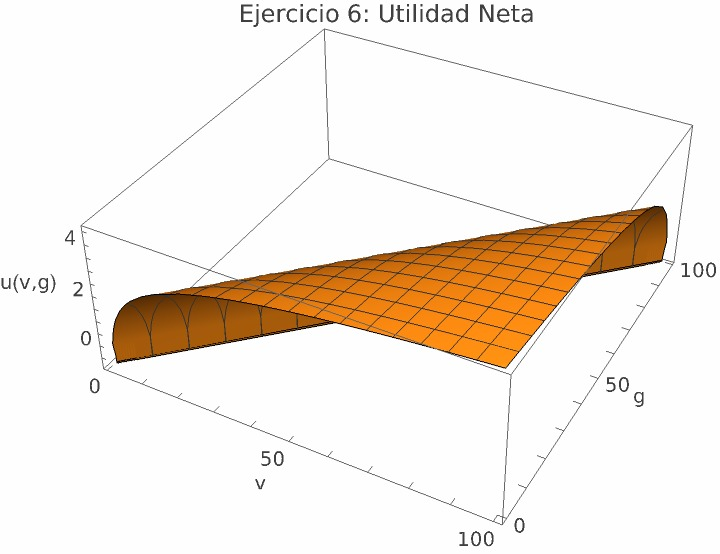
\includegraphics[width=0.75\textwidth]{images/Ejercicio6.png}
\end{center}

\newpage

% ---------------- Ejercicio 7 ----------------
\section*{Ejercicio 7: El ``Filtro de Ruido Gaussiano'' (Exponencial)}
\[ f(x,y) = e^{-(x^2+y^2)} \]

\textbf{Representación Verbal:} El peso del desenfoque es máximo (1) en el píxel origen y disminuye exponencialmente con la distancia radial a este.

\textbf{Variables:}
\begin{itemize}[nosep]
    \item Independientes: $x$ (Distancia X), $y$ (Distancia Y)
    \item Dependiente: $f(x,y)$ (Intensidad de desenfoque)
\end{itemize}

\textbf{Dominio y Rango:}
\begin{itemize}[nosep]
    \item Dominio: $D = \mathbb{R}^2$ (Todo el plano cartesiano)
    \item Rango: $R = (0, 1]$
\end{itemize}

\textbf{Representación Algorítmica (Tabular):} \quad $z = e^{-(x^2+y^2)}$

\begin{center}
\begin{tabular}{ccc}
\toprule
$x$ & $y$ & $f(x,y)$ \\
\midrule
0 & 0 & 1.000 \\
1 & 0 & $e^{-1} \approx 0.368$ \\
1 & 1 & $e^{-2} \approx 0.135$ \\
\bottomrule
\end{tabular}
\end{center}

\begin{center}
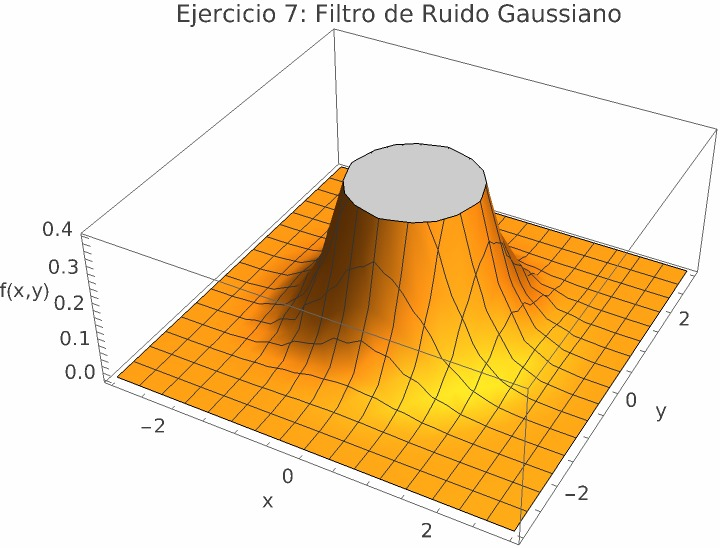
\includegraphics[width=0.75\textwidth]{images/Ejercicio7.png}
\end{center}

\newpage

% ---------------- Ejercicio 8 ----------------
\section*{Ejercicio 8: Zona de Tracking en VR (Paraboloide)}
\[ Z(x,y) = x^2 + y^2 \]

\textbf{Representación Verbal:} La pérdida de precisión del sensor tracking es nula en el origen y crece cuadráticamente conforme el usuario se aleja del centro.

\textbf{Variables:}
\begin{itemize}[nosep]
    \item Independientes: $x$ (Desplazamiento X), $y$ (Desplazamiento Y)
    \item Dependiente: $Z$ (Pérdida de precisión)
\end{itemize}

\textbf{Dominio y Rango:}
\begin{itemize}[nosep]
    \item Dominio: $D = \mathbb{R}^2$
    \item Rango: $R = [0, \infty)$
\end{itemize}

\textbf{Representación Algorítmica (Tabular):} \quad $Z = x^2+y^2$

\begin{center}
\begin{tabular}{ccc}
\toprule
$x$ & $y$ & $Z(x,y)$ \\
\midrule
0 & 0 & 0 \\
1 & 2 & 5 \\
3 & 4 & 25 \\
\bottomrule
\end{tabular}
\end{center}

\begin{center}
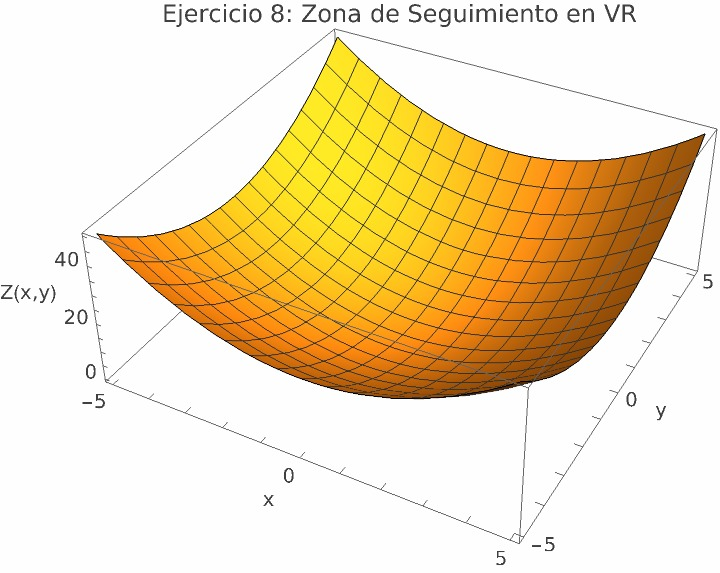
\includegraphics[width=0.75\textwidth]{images/Ejercicio8.png}
\end{center}

\newpage

% ---------------- Ejercicio 9 ----------------
\section*{Ejercicio 9: El ``Costo de Almacenamiento'' (Suma de Raíces)}
\[ f(x,y) = \sqrt{x} + \sqrt{y} \]

\textbf{Representación Verbal:} El costo total de infraestructura incrementa de manera sublineal según las unidades adquiridas de almacenamiento y cómputo.

\textbf{Variables:}
\begin{itemize}[nosep]
    \item Independientes: $x$ (Almacenamiento), $y$ (Cómputo)
    \item Dependiente: $f(x,y)$ (Costo total)
\end{itemize}

\textbf{Dominio y Rango:}
\begin{itemize}[nosep]
    \item Dominio: $D = \{(x,y) \in \mathbb{R}^2 \mid x \geq 0,\ y \geq 0\}$
    \item Rango: $R = [0, \infty)$
\end{itemize}

\textbf{Representación Algorítmica (Tabular):} \quad $z = \sqrt{x}+\sqrt{y}$

\begin{center}
\begin{tabular}{ccc}
\toprule
$x$ & $y$ & $f(x,y)$ \\
\midrule
0 & 0 & 0 \\
4 & 9 & $2+3=5$ \\
16 & 25 & $4+5=9$ \\
\bottomrule
\end{tabular}
\end{center}

\begin{center}
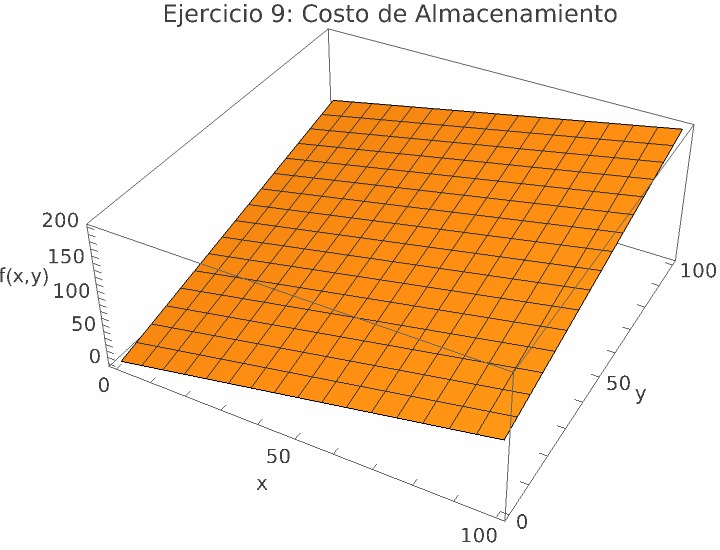
\includegraphics[width=0.75\textwidth]{images/Ejercicio9.png}
\end{center}

\newpage

% ---------------- Ejercicio 10 ----------------
\section*{Ejercicio 10: Tasa de Conversión en E-commerce (Exponencial)}
\[ T(u,s) = 1 - e^{-(u+s)} \]

\textbf{Representación Verbal:} La probabilidad de compra se incrementa asintóticamente hacia 1 (100\%) conforme aumenta la inversión combinada en UX y SEO.

\textbf{Variables:}
\begin{itemize}[nosep]
    \item Independientes: $u$ (Inversión UX), $s$ (Inversión SEO)
    \item Dependiente: $T$ (Probabilidad de compra)
\end{itemize}

\textbf{Dominio y Rango:}
\begin{itemize}[nosep]
    \item Dominio: $D = \{(u,s) \in \mathbb{R}^2 \mid u \geq 0,\ s \geq 0\}$
    \item Rango: $R = [0, 1)$
\end{itemize}

\textbf{Representación Algorítmica (Tabular):} \quad $T = 1 - e^{-(u+s)}$

\begin{center}
\begin{tabular}{ccc}
\toprule
$u$ (\$) & $s$ (\$) & $T(u,s)$ \\
\midrule
0 & 0 & 0.000 (0\%) \\
1 & 0 & $1-e^{-1} \approx 0.632$ (63.2\%) \\
1 & 1 & $1-e^{-2} \approx 0.865$ (86.5\%) \\
\bottomrule
\end{tabular}
\end{center}

\begin{center}
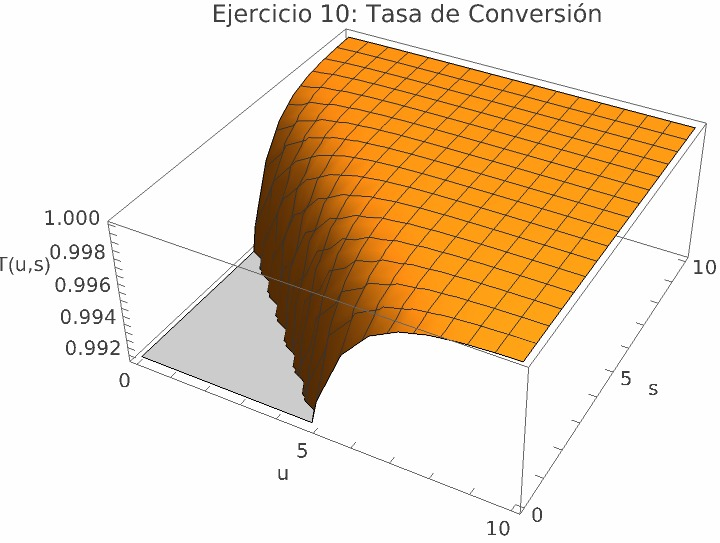
\includegraphics[width=0.75\textwidth]{images/Ejercicio10.png}
\end{center}

\end{document}